\documentclass[tikz]{standalone}
\usepackage{pgfplots}
\pgfplotsset{compat=1.15}
\usepackage{mathrsfs}
\usetikzlibrary{arrows,calc}
\usepackage{tkz-euclide}

\pagestyle{empty}

\definecolor{AngleClr}{rgb}{0,0.39215686274509803,0}
\definecolor{ShapeClr}{rgb}{0.6,0.2,0}
\definecolor{BlueClr}{RGB}{13,93,184}
\definecolor{RedClr}{RGB}{150,36,8}

\begin{document}

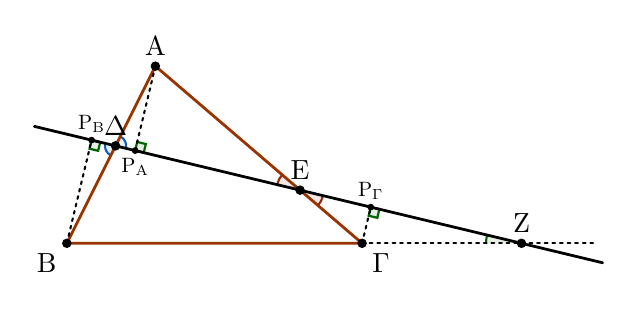
\begin{tikzpicture}[scale=.75]
\tkzSetUpLine[line width=1pt,color=black]
\tkzSetUpPoint[fill=black]

\tkzDefPoints{0/0/B,1.5/3/A,5/0/C}

\tkzDefPointOnLine[pos=0.45](A,B)\tkzGetPoint{D}
\tkzDefPointOnLine[pos=0.7](A,C)\tkzGetPoint{E}

\tkzDefPointBy[projection=onto D--E](A)\tkzGetPoint{PA}
\tkzDefPointBy[projection=onto D--E](B)\tkzGetPoint{PB}
\tkzDefPointBy[projection=onto D--E](C)\tkzGetPoint{PC}

\tkzInterLL(D,E)(B,C)\tkzGetPoint{Z}

\tkzFillPolygon[fill=white](A,B,C)

\tkzFillAngles[fill=BlueClr,size=.18,fill opacity=0.1](PB,D,B PA,D,A)
\tkzMarkAngles[line width=0.75pt,size=.18,color=BlueClr](PB,D,B PA,D,A)

\tkzFillAngles[fill=RedClr,size=.4,fill opacity=0.1](A,E,PA C,E,PC)
\tkzMarkAngles[line width=0.75pt,size=.4,color=RedClr](A,E,PA C,E,PC)

\tkzFillAngles[fill=AngleClr,size=.6,fill opacity=0.1](E,Z,C)
\tkzMarkAngles[line width=0.75pt,size=.6,color=AngleClr](E,Z,C)

\tkzMarkRightAngles[line width=0.8pt, size=.15,color=AngleClr,fill=AngleClr,fill opacity=0.1](A,PA,E B,PB,E C,PC,Z)

\tkzDrawPolygon[color=ShapeClr](A,B,C)

\tkzDrawSegments[line width=1pt,color=black,add=0.2 and 0.2](D,Z)
\tkzDrawSegments[line width=0.75pt,color=black,dashed,dash pattern=on 1pt off 1.75pt](A,PA B,PB C,PC)
\tkzDrawSegments[line width=0.75pt,color=black,dashed,dash pattern=on 1pt off 1.75pt,add=0 and 0.45](C,Z)



\tkzDrawPoints[size=3](A,B,C,E,D,Z)
\tkzDrawPoints[size=2](PA,PB,PC)
\tkzLabelPoint[above](A){$\rm A$}
\tkzLabelPoint[below left](B){$\rm B$}
\tkzLabelPoint[below right](C){$\rm \Gamma$}
\tkzLabelPoint[above](D){$\rm \Delta$}
\tkzLabelPoint[above](E){$\rm E$}
\tkzLabelPoint[above](Z){$\rm Z$}

\tkzLabelPoint[below,scale=0.75](PA){$\rm P_A$}
\tkzLabelPoint[above,scale=0.75](PB){$\rm P_B$}
\tkzLabelPoint[above,scale=0.75](PC){$\rm P_\Gamma$}

\end{tikzpicture}

\end{document}
